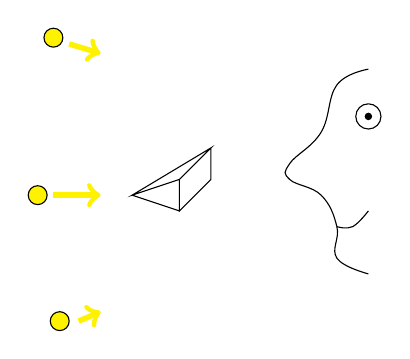
\begin{tikzpicture}[scale=0.4]
% La camera
\path[draw] (-0.5,0)--(1,-0.5)--(1,0.5)--(-0.5,0)--(2,1.5)--(1,0.5)--(1,-0.5)--(2,0.5)--(2,1.5);

% Les trois soleils
\uncover<2->{
\draw[fill=yellow] (-3,5) circle(0.3);
\draw[->,line width=2pt, yellow] (-2.5,4.8)--(-1.5,4.5);
}
\uncover<3->{
\draw[fill=yellow] (-3.5,0) circle(0.3);
\draw[->,line width=2pt, yellow] (-3,0)--(-1.5,0);
}
\uncover<4->{
\draw[fill=yellow] (-2.8,-4) circle(0.3);
\draw[->,line width=2pt, yellow] (-2.2,-4)--(-1.5,-3.7);
}



% Contour d'une tete
\draw  plot[smooth, tension=.7] coordinates {(7,4) (6,3.5) (5.5,2) (4.5,1) (4.5,0.5) (5.5,0) (6,-1) (6,-2) (7,-2.5)};
% Yeux
\draw (7,2.5) circle(0.4);
\draw[fill] (7,2.5) circle(0.1);
% Bouche
\draw  plot[smooth, tension=.7] coordinates {(6,-1) (6.5,-1) (7,-0.5)};

\end{tikzpicture}